\documentclass[aspectratio=169]{beamer}
\setbeamertemplate{caption}[numbered]
\usepackage{outlines}
\usepackage{graphicx}
\usepackage{float}
\usepackage{amsfonts}
\usepackage{mhchem}
\usepackage{cite}
\usepackage{lmodern}
\usepackage{amsrefs}
\usepackage{amsmath}
\usepackage{amssymb}
\usepackage{hyperref}
\usepackage{listings}
\usepackage{ccicons}
\usetheme{Madrid}
\usecolortheme[RGB={30, 80, 59}]{structure}
\title{Python for High-Performance Computing}
\author{Stephen Szwiec}
\institute[CCAST]{Center for Computationally Assisted Science and Technology}
\date{\today}
\newlength{\sepwidth}
\newlength{\colwidth}
\setlength{\sepwidth}{0.010\linewidth}
\setlength{\colwidth}{0.5\linewidth}
\newcommand{\separatorcolumn}{\begin{column}{\sepwidth}\end{column}}

\beamertemplatenavigationsymbolsempty

\begin{document}

	\frame{\titlepage}

    \begin{frame}{Outline}
        \begin{outline}
            \1 Presentation 
            \1 Live Demo 
            \1 Open Discussion and Questions
        \end{outline}
    \end{frame}

     \begin{frame}{Outline}
        \begin{outline}
            \1 Introduction
            \1 The Shell and Shell Commands 
            \1 Environment Variables
            \1 History of HPC to Python
                \2 High-Level Languages
                \2 Why Python?
            \1 Python for HPC
                \2 Python and Package Management
                \2 Using \texttt{pip}
                \2 Using \texttt{conda}
            \1 Successful Python on HPC
        \end{outline}
    \end{frame}

    \begin{frame}{Introduction}
        \centering
        \Huge How did we get here?
    \end{frame}

    \begin{frame}{Introduction}
        \begin{figure}[H]
            \centering
            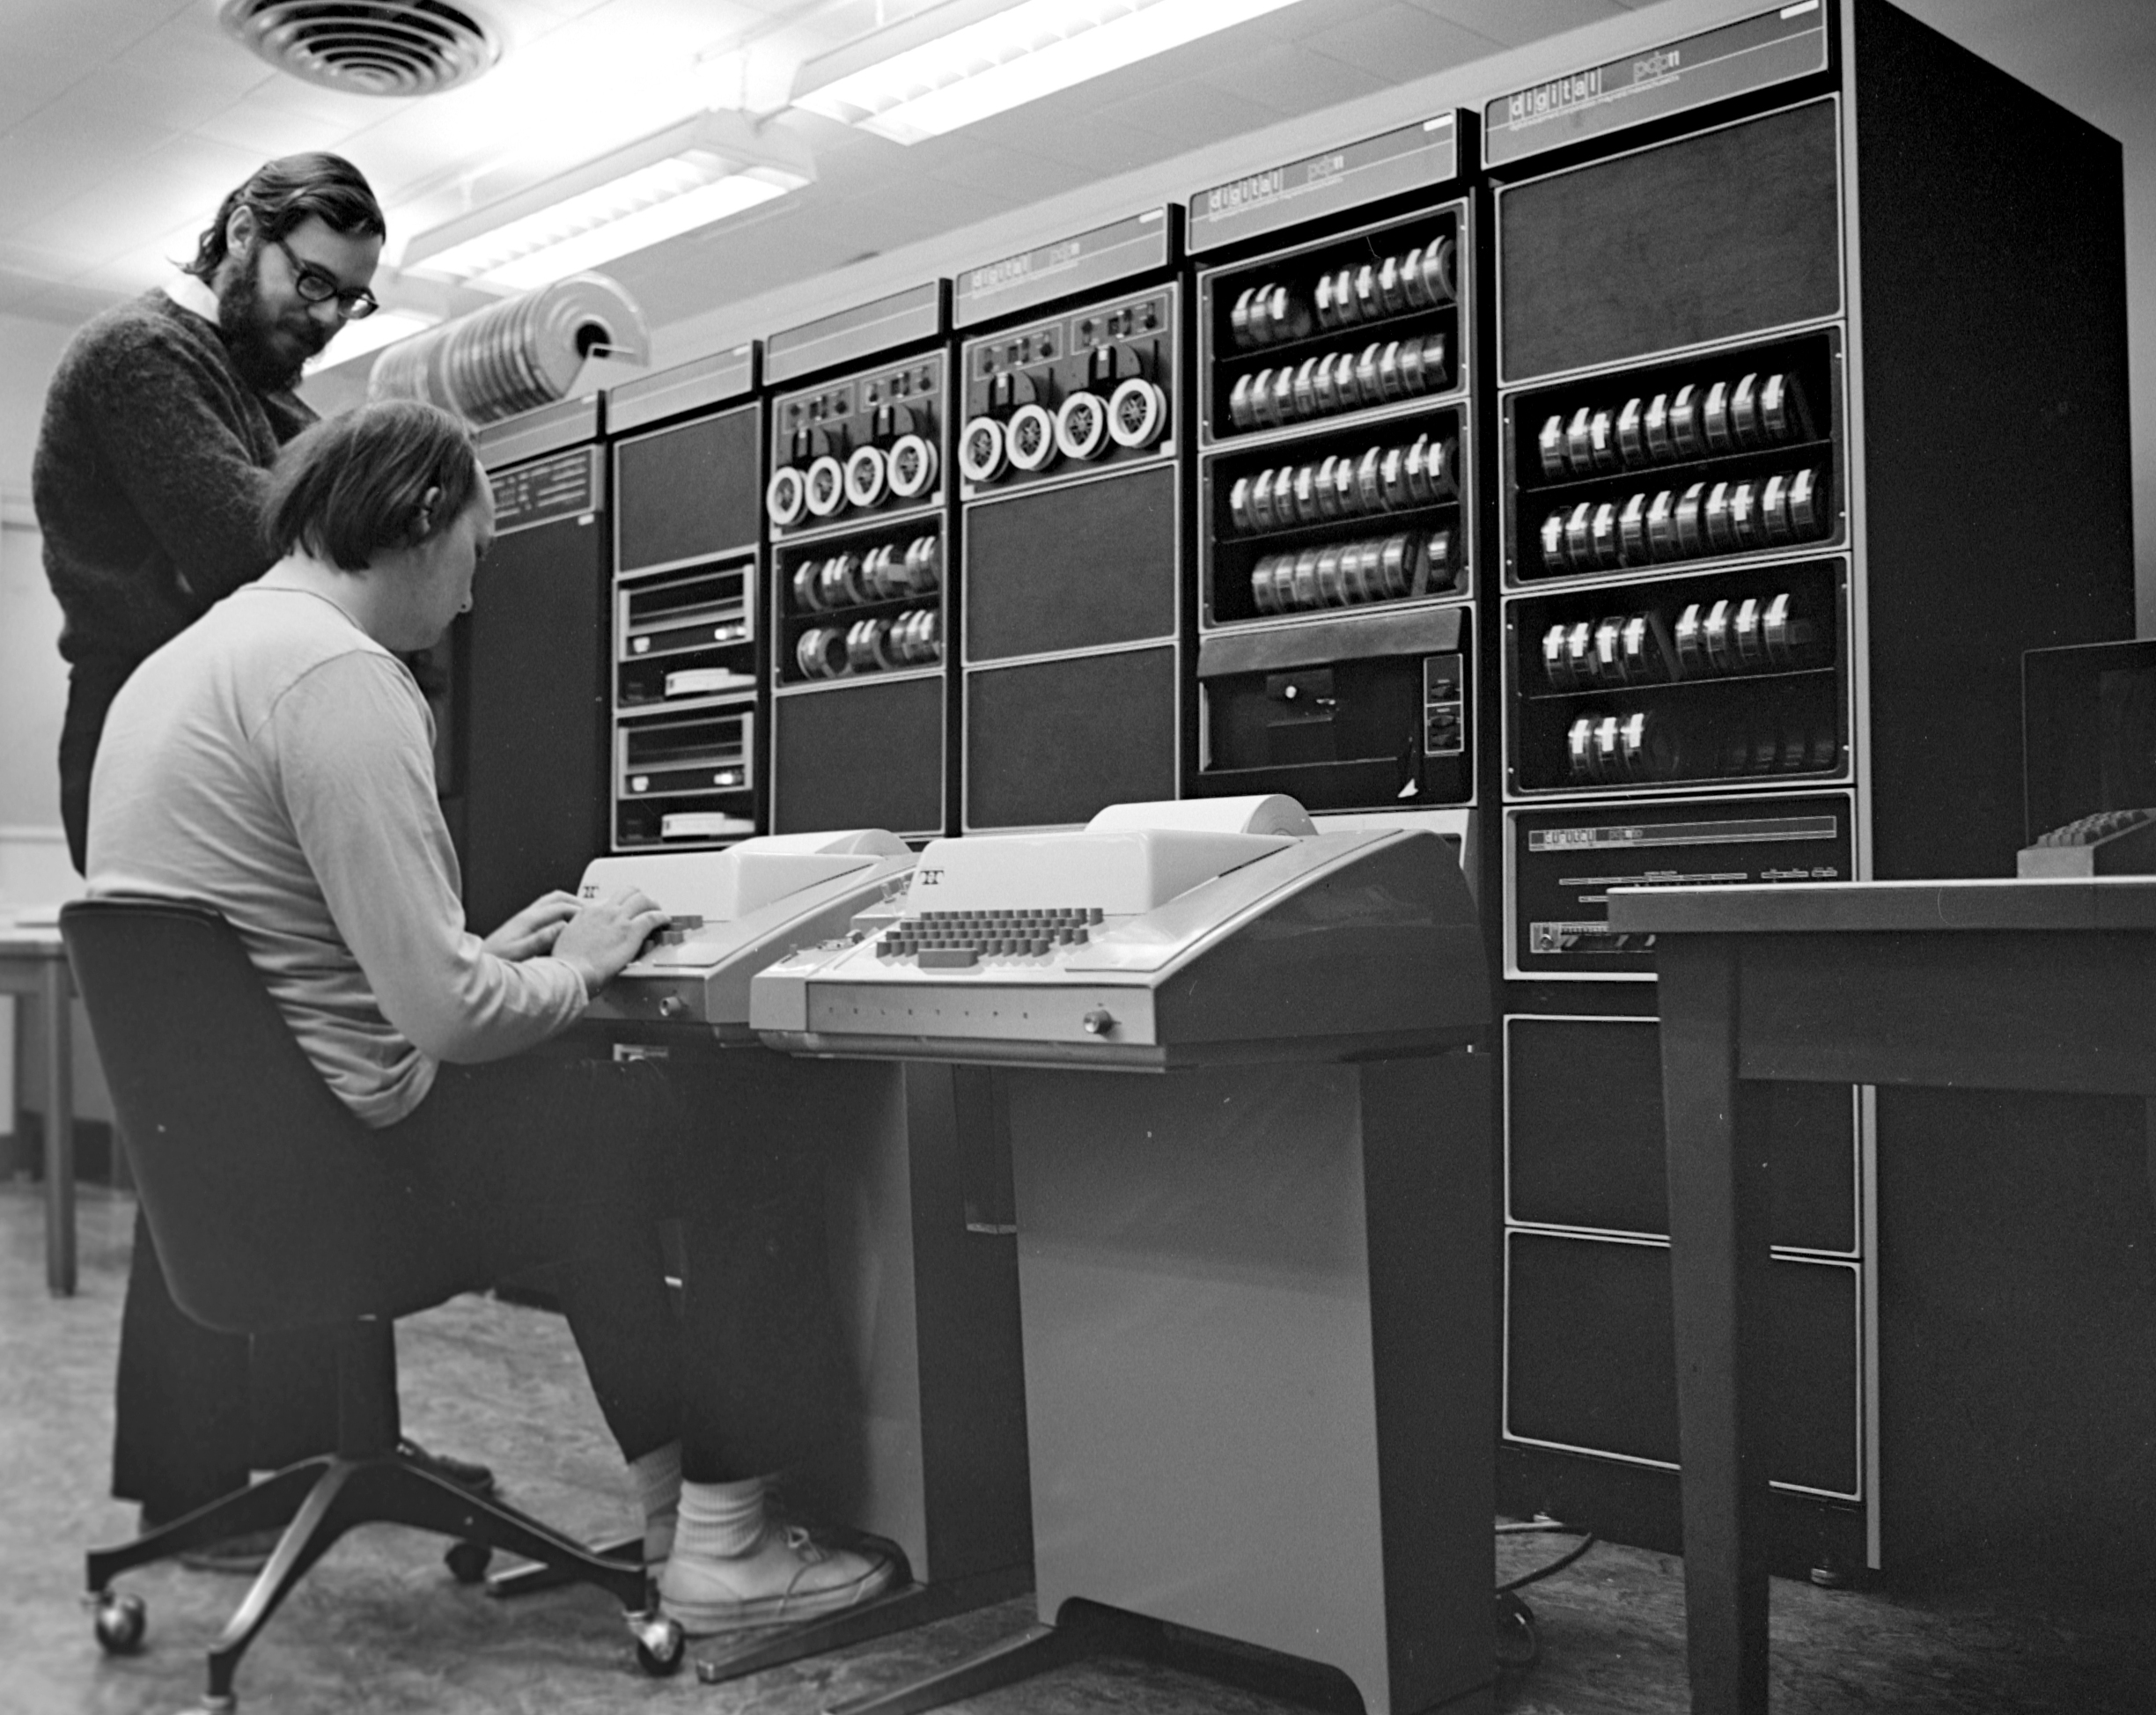
\includegraphics[width=0.50\linewidth]{kenanddennis.jpg}
            \caption{Ken Thompson and Dennis Ritchie at Bell Labs, circa 1970. \ccLogo Peter Hamer, 2011.}
        \end{figure}
    \end{frame}

    \begin{frame}{Introduction}
        \begin{outline}
            \1 Unix-like operating systems are the most common operating systems used in both academia and industry for scientific computing.
            \2 Unix was developed at Bell Labs in the 1970s by Ken Thompson, Dennis Ritchie, and others. 
            \2 Efforts by the Free Software Foundation and Linus Torvalds led to the development of Linux in the 1990s. 
            \1 Linux is a Unix-like operating system, and shares common ideas with Unix (BSD, MacOS, iOS, etc.)
                \2 Linux is also the basis for Android.
        \end{outline}
    \end{frame}

    \begin{frame}{Introduction}
        \begin{columns}
            \begin{column}{0.5\linewidth}
                \begin{figure}[H]
                    \centering
                    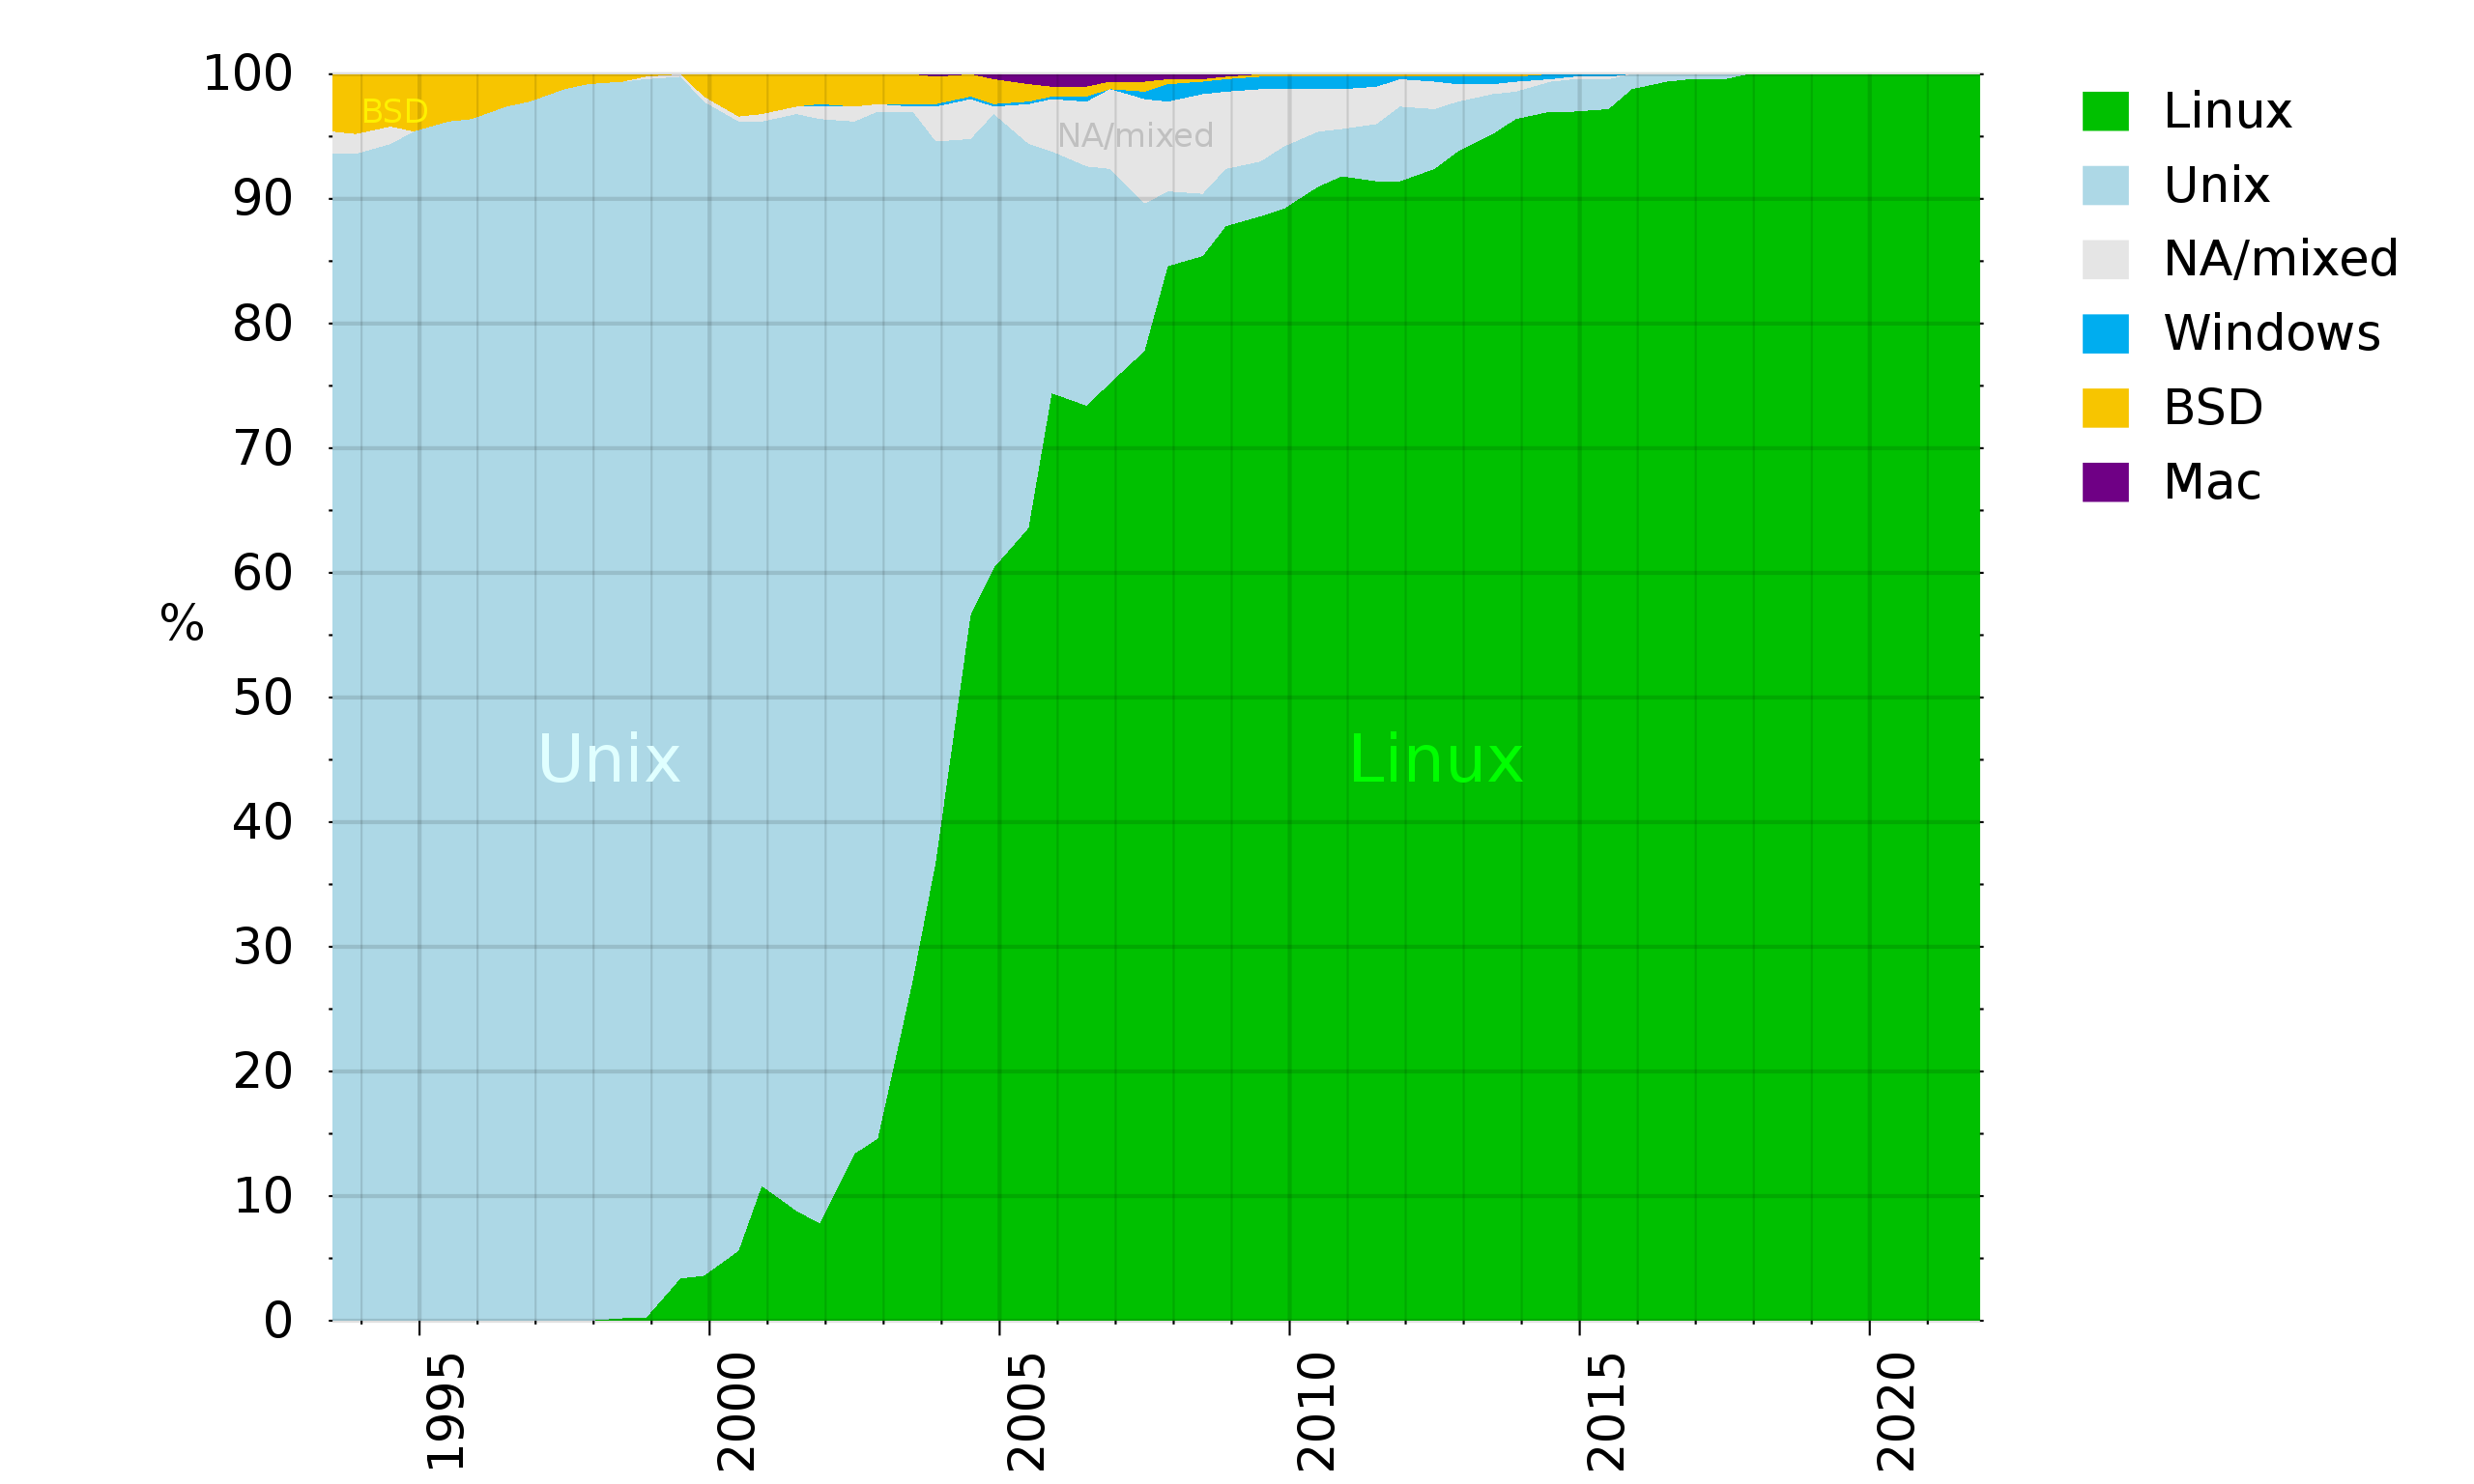
\includegraphics[width=\linewidth]{top500.png}
                    \caption{Top 500 Supercomputers, by operating system, 1993--2021 \ccPublicDomain Benedikt Seidl, 2021.}
                \end{figure}
            \end{column}
            \begin{column}{0.5\linewidth}
                \begin{outline}
                \1 Together, Unix and Linux:
                    \2 99\% of smartphones
                    \2 31\% of personal computers
                    \2 80\% of servers
                    \2 100\% of TOP500 supercomputers
                \1 Familiarity with these systems is essential for scientific computing, cloud computing, high-performance computing, and mobile development.
            \end{outline}
            \end{column}
        \end{columns}
    \end{frame}

    \begin{frame}{Introduction}
        \begin{columns}
            \begin{column}{0.5\linewidth}
                \begin{figure}[H]
                    \centering
                    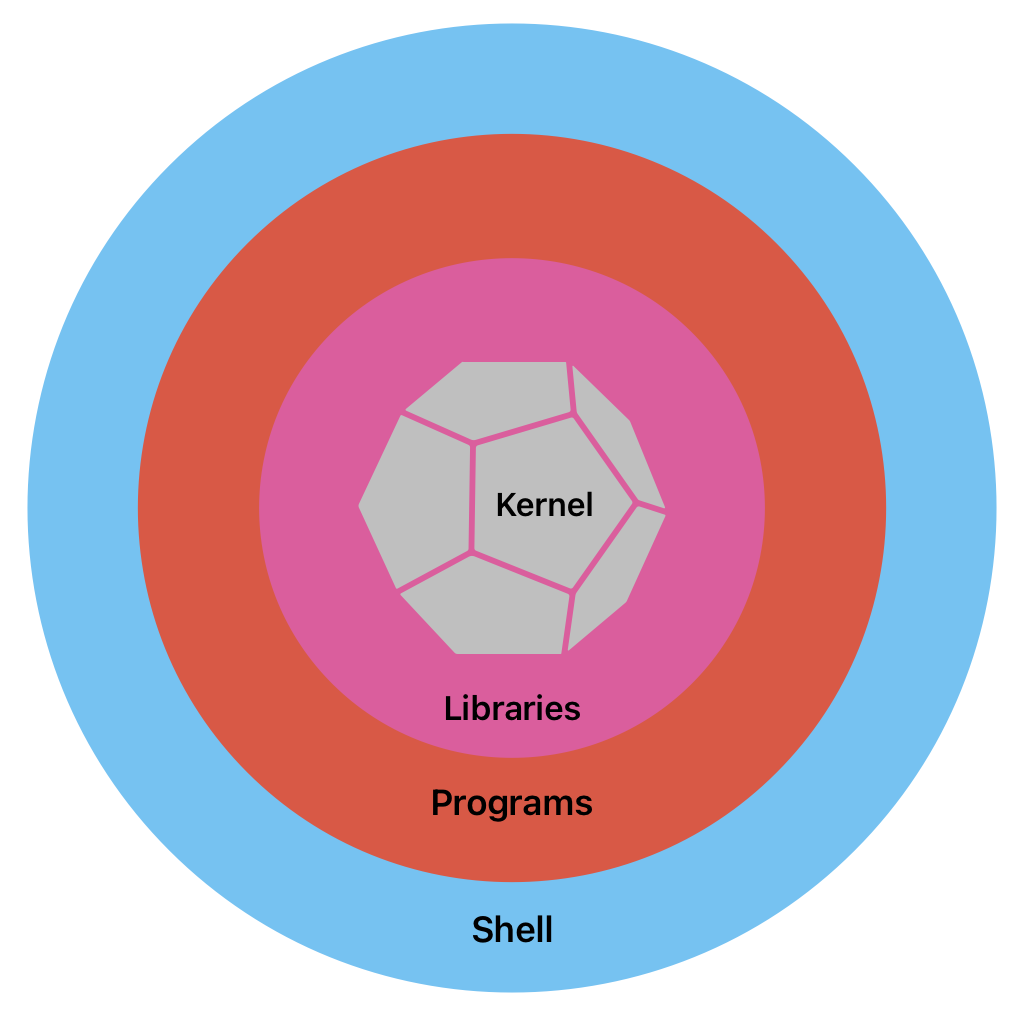
\includegraphics[width=0.7\linewidth]{kernel.png}
                    \caption{An idealized view of the Unix-like operating system.}
                \end{figure}
            \end{column}
            \begin{column}{0.5\linewidth}
                \begin{outline}
                    \1 The Unix-like operating system is composed of three main parts:
                        \2 \textbf{Kernel:} the core of the operating system, which manages the hardware.
                        \2 \textbf{Libraries:} abstract interfaces to the kernel, which provide common functionality.
                        \2 \textbf{Programs:} use the libraries to perform tasks.
                        \2 \textbf{Shell:} a command-line interface to the operating system. 
                    \1 The shell is the primary interface to the operating system.
                \end{outline}
            \end{column}
        \end{columns}
    \end{frame}

    \begin{frame}{The Shell and Shell Commands}
        \begin{figure}[H]
            \centering
            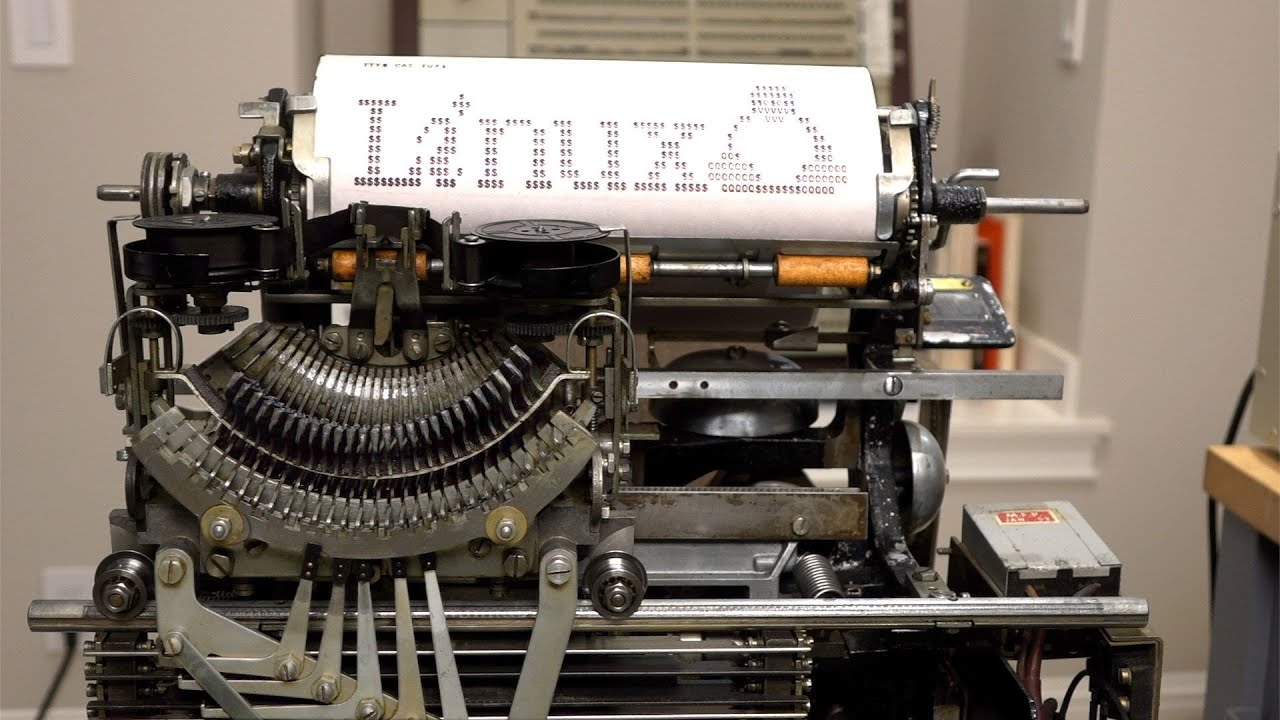
\includegraphics[width=0.70\linewidth]{tty}
            \caption{A 1930s Teletypewriter, connected to a modern Linux system via SSH. © CuriousMarc, 2020 [https://youtu.be/2XLZ4Z8LpEE]}
        \end{figure}
    \end{frame}

    \begin{frame}{The Shell and Shell Commands}
        \begin{outline}
            \1 The shell is a command-line interface to the operating system.
                \2 The shell is a program that interprets commands and executes them.
                \2 The shell is also a Turing-complete scripting language.
            \1 The shell is the primary interface to the operating system.
                \2 Implements a read-eval-print loop (REPL.) 
        \end{outline}
    \end{frame}

    \begin{frame}{The Shell and Shell Commands}
        \begin{outline}
            \1 Shell scripts can be used to automate tasks, and are often used to run programs on high-performance computing clusters.
            \1 Quick example: script to create a series of numbered directories: 
            \0 \texttt{\$ for i in \{1..10\}; do mkdir \$i; done}
        \end{outline}
    \end{frame}

    \begin{frame}{Environment Variables} 
        \begin{outline}
            \1 If the shell is just a type-and-run interface, how does the shell \textit{know} what to do?
                \2 \texttt{\$ which mkdir} 
            \1 The shell uses environment variables to store information about the system and the user:
                \2 Environment variables are key-value pairs that are used by the shell and programs to determine how to behave.
                \2 In the above example, we set a variable \texttt{i} to a value from 1 to 10, and called it with \texttt{\$i}.
        \end{outline}
    \end{frame}

    \begin{frame}{Environment Variables}
        \begin{outline}
            \1 Common environment variables:
                \2 \texttt{\$PATH} 
                \2 \texttt{\$LD\_LIBRARY\_PATH} 
                \2 \texttt{\$HOME} 
            \1 Worth noting for CCAST Portable Batch System (PBS) jobs: 
                \2 \texttt{\$SCRATCH} 
                \2 \texttt{\$PBS\_NODEFILE}
                \2 \texttt{\$PBS\_O\_WORKDIR}
            \1 Environment variables can be set, unset, and used in the shell:
                \2 \texttt{\$ export VARIABLE=value}
                \2 \texttt{\$ unset VARIABLE} 
                \2 \texttt{\$ echo \$VARIABLE}
                \2 \texttt{\$ echo \$\{VARIABLE\}}
        \end{outline}
    \end{frame}

    \begin{frame}{Environment Variables}
        \begin{outline}
            \1 On an HPC cluster, there are many different software packages installed. 
                \2 Some software packages are incompatible with others.
            \1 Environment modules are used to manage software packages on an HPC cluster:
                \2 set environment variables for a specific software package.
                \2 can be loaded and unloaded as needed.
            \0 \texttt{\$ module load cuda/12.3} 
                \1 loads the CUDA 12.3 environment module on the cluster
                \1 just sets \texttt{\$PATH} and \texttt{\$LD\_LIBRARY\_PATH}.
        \end{outline}
    \end{frame}

    \begin{frame}{Environment Variables}
        \centering
        \Huge The shell is a scripting language,\\
        environment variables are part of the language.
    \end{frame}

    \begin{frame}{History of HPC to Python}
        \begin{figure}[H]
            \centering
            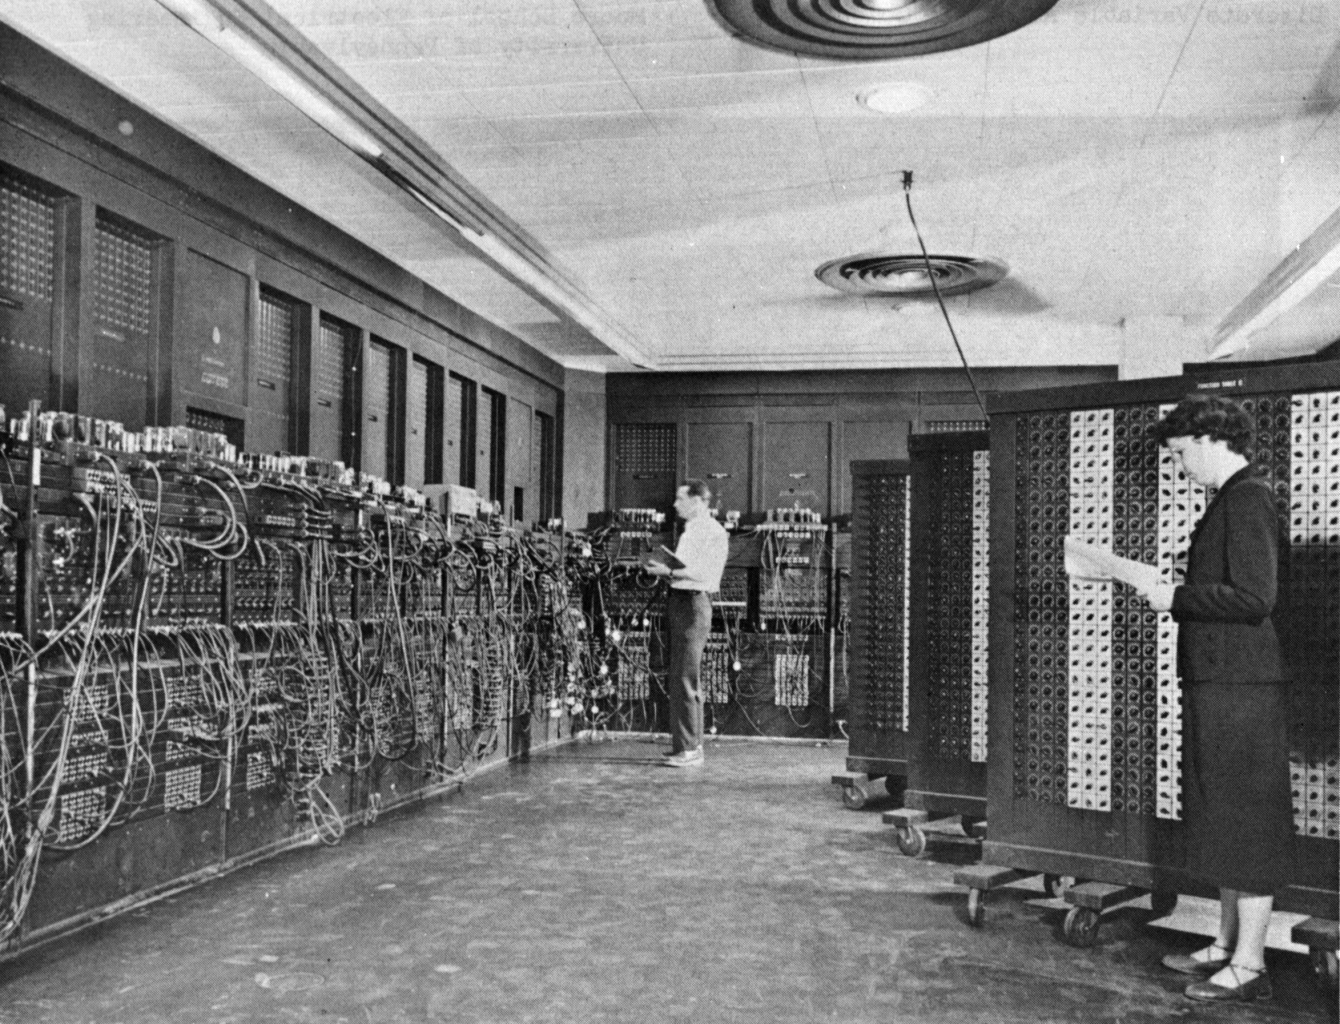
\includegraphics[width=0.50\linewidth]{ENIAC.jpg}
            \caption{The ENIAC computer, ran between 1947 -- 1955. \ccLogo Public Domain, US Army, 1947.}
        \end{figure}
    \end{frame}
    
    \begin{frame}{History of HPC to Python}
        \begin{outline}
            \1 High-performance computing has a long history, dating back to the 1940s with the development of the ENIAC computer.
                \2 Problem fields: ballistics, weather forecasting, nuclear physics, fluid dynamics, etc. 
                \2 All using linear algebraic discrete methods to solve partial differential equations: floating point approximations of continuous mathematics.
            \1 Original 'programming' done by directly manipulating the hardware, setting registers, etc. 
                \2 First programming language using instructions: Grace Hopper's 1952 A-0 System. 
        \end{outline}
    \end{frame}

    \begin{frame}{History of HPC to Python}
        \begin{figure}[H]
            \centering
            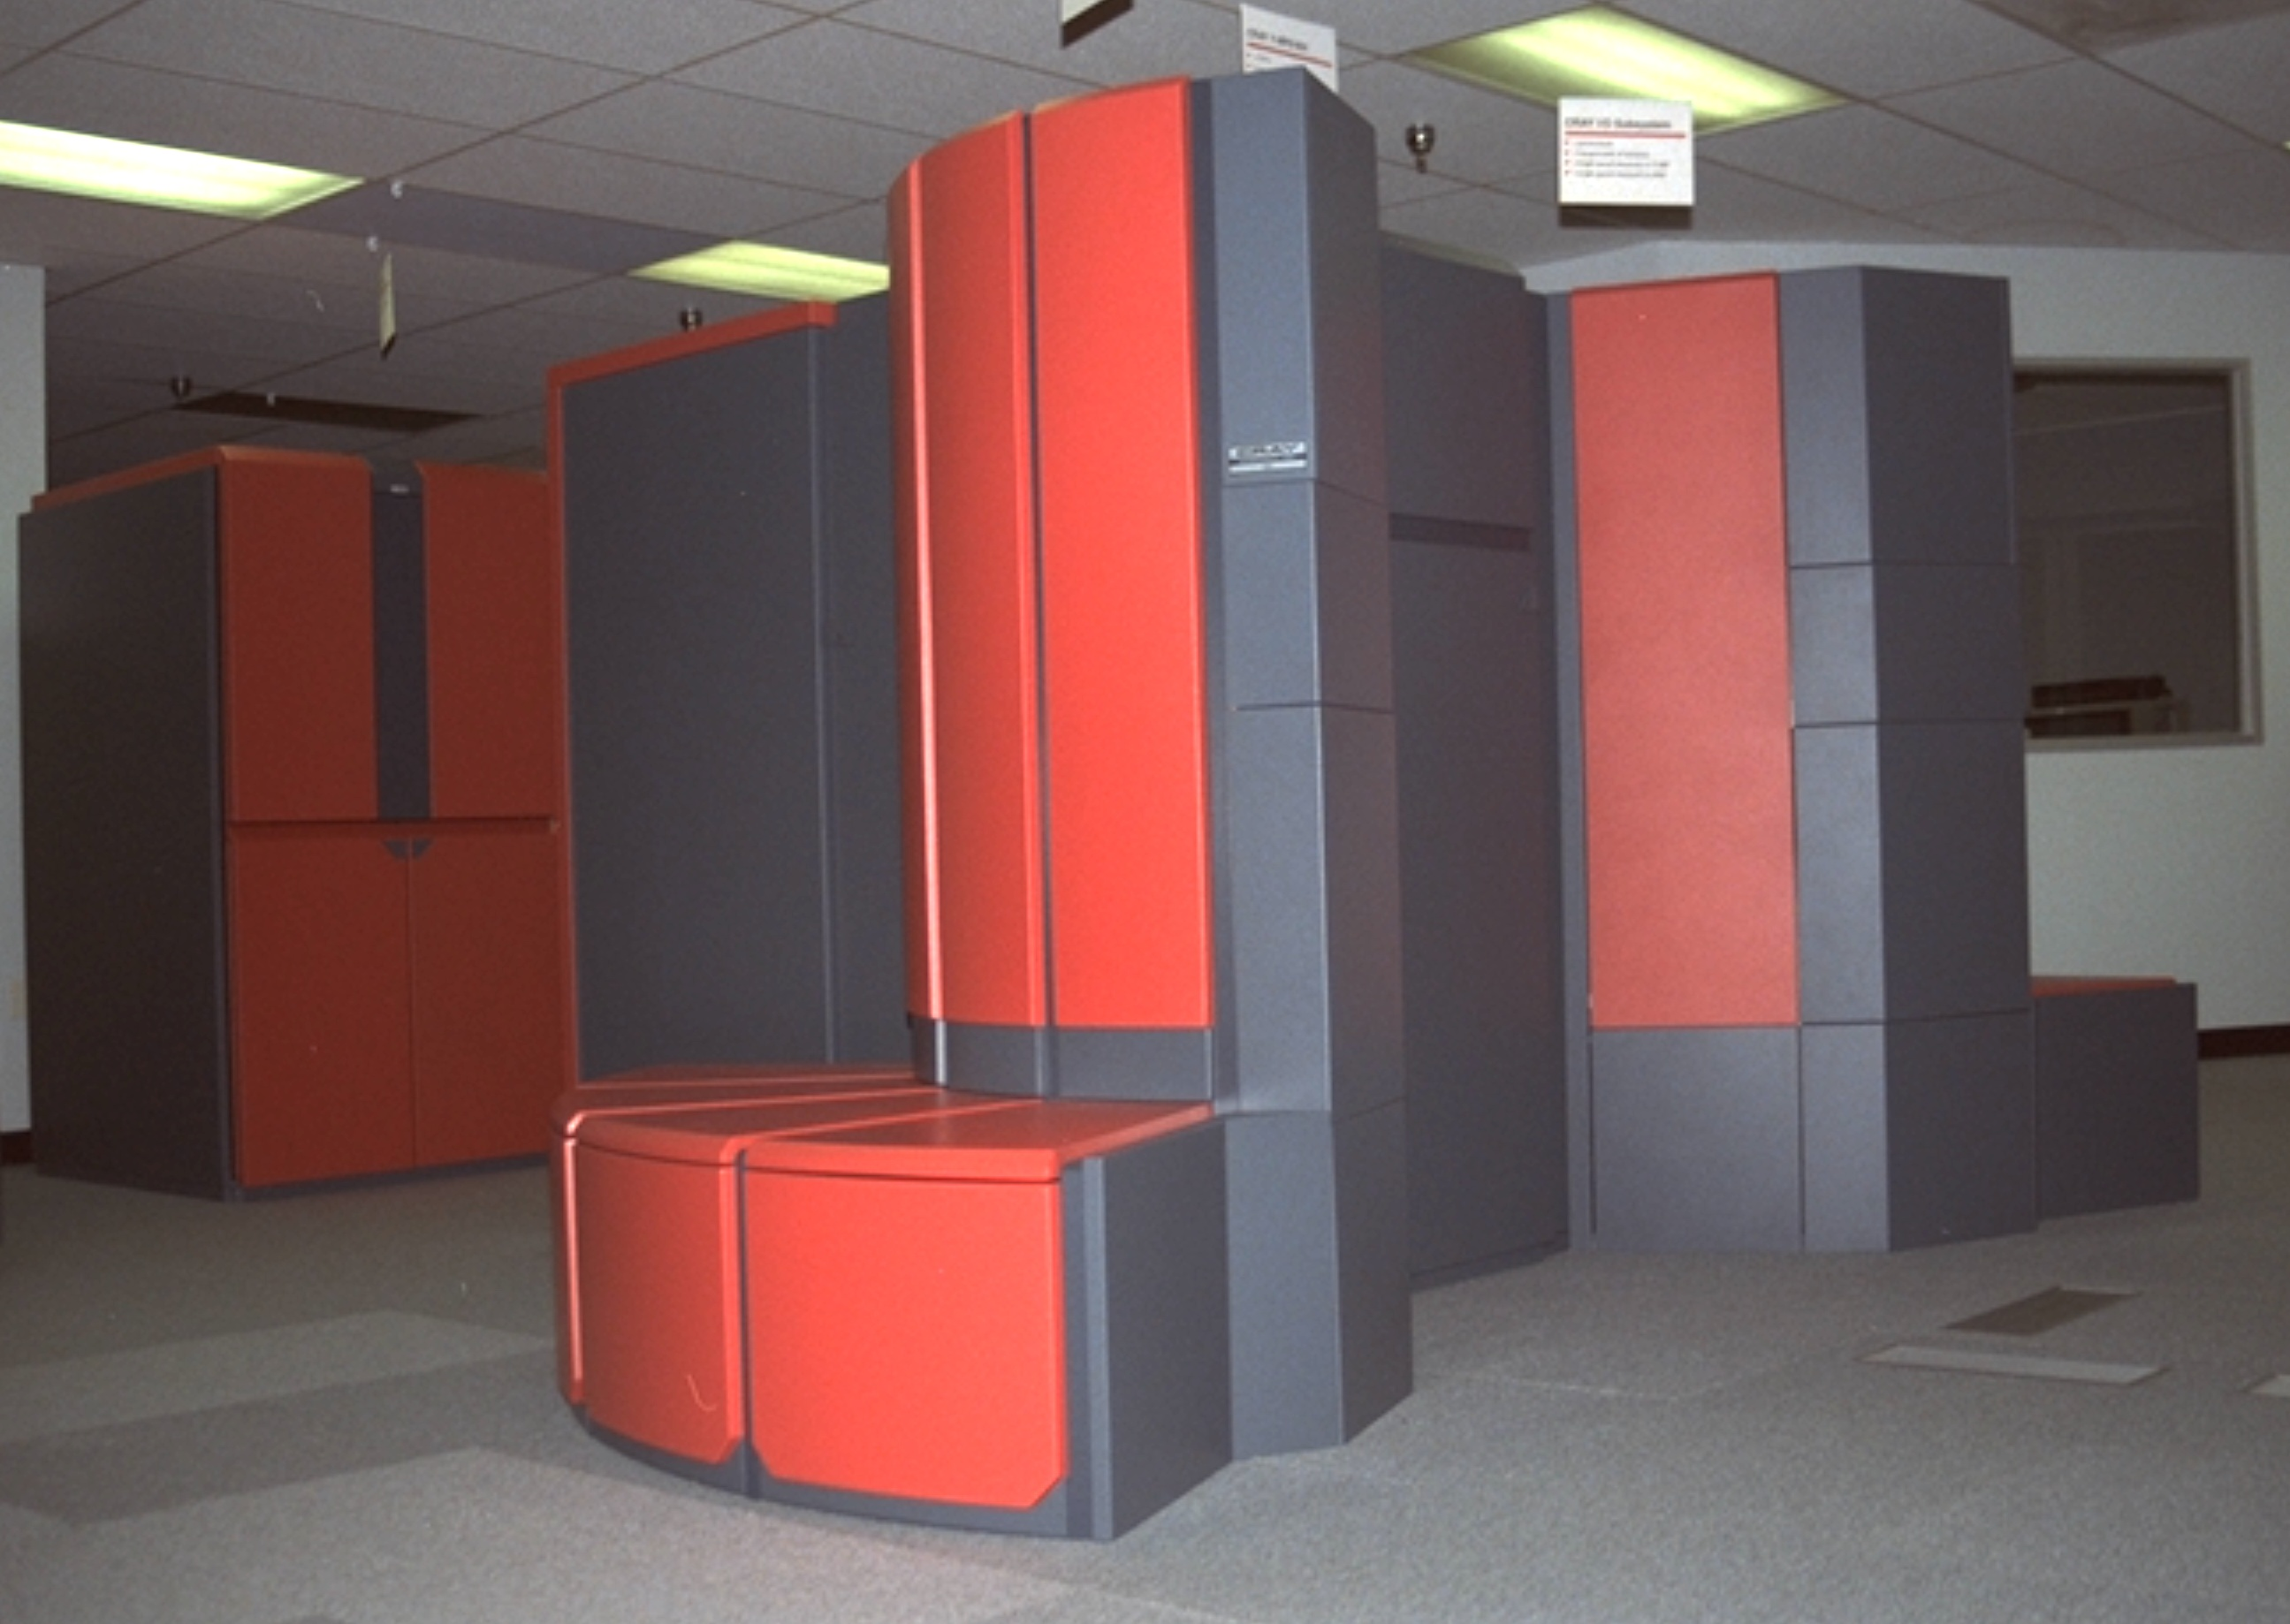
\includegraphics[width=0.50\linewidth]{Cray.jpg}
            \caption{Cray Y-MP Supercomputer, ran between 1988 -- 1990 at NASA Center for Computational Sciences. \ccLogo Dave Pape}
        \end{figure}
    \end{frame}

    \begin{frame}{History of HPC to Python}
        \begin{outline}
            \1 The development of high-level programming languages in the 1950s and 1960s allowed for more complex programs to be written.
                \2 \textbf{FORTRAN}, developed by IBM in 1957, was the first high-level programming language.
                \2 followed by \textbf{C} (and later, \textbf{C++}.)
            \1 With these, the workflow of scientific computing changed:
                \2 Write code and compile it for the target system
                \2 Run the code on the computer using the shell or a batch scheduler
                \2 Analyze the results using a separate program
            \1 These languages are still used today, especially where performance is critical:
                \2 Still the basis for scientific computing libraries: eg. \textbf{NumPy} (C), \textbf{SciPy} (Fortran,C++)
        \end{outline}
    \end{frame}

    \begin{frame}{History of HPC to Python}
        \begin{figure}[H]
            \centering
            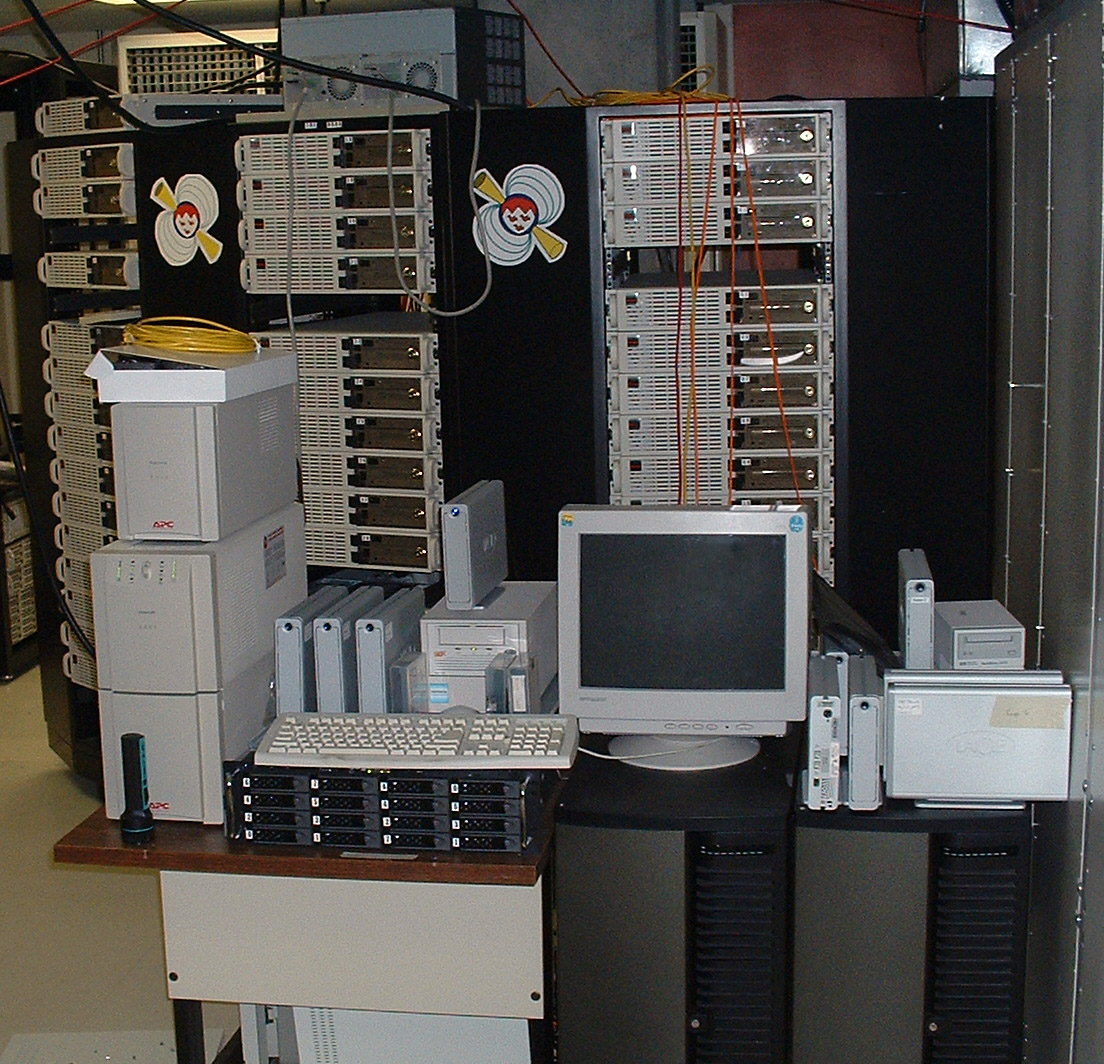
\includegraphics[width=0.40\linewidth]{Borg.jpg}
            \caption{The Borg cluster, a 52-node system run by the McGill University pulsar group. \ccLogo McGill University, 2014.}
        \end{figure}
    \end{frame}

    \begin{frame}{History of HPC to Python}
        \begin{outline}
            \1 During the 1990s:
                \2 Hardware costs decreased and PC (x86) computers become plentiful, leading to the development of commodity clusters.
                \2 The development of the Message Passing Interface (MPI) standard for parallel computing.
                \2 GPUs are originally developed to make games run better: use matrix operations to render 3D graphics. 
                \2 The development of low-performance languages for scripting and web development: Perl, PHP, Ruby, and... 
        \end{outline}
    \end{frame}

    \begin{frame}{Why Python?}
        \begin{outline}
            \1 1991 - Python 0.9.0 is released by Guido van Rossum. 
                \2 Originally for scripting system administration tasks on the Amoeba distributed operating system.
                \2 Python is a high-level, interpreted, general-purpose programming language.
                \2 Guido wanted to create a language that was easy to read and write, and that was extensible.
                    \3 "Python is a language that emphasizes readability and simplicity, with a focus on pragmatic use and ease of learning." -- Van Rossum
            \1 Python today is explosively popular:
                \2 2nd most popular language on GitHub.
                \2 1st most popular language for data science.
                \2 1st most popular language for machine learning.
        \end{outline}
    \end{frame}

    \begin{frame}{Why Python?}
        \centering
        \Huge Python must be so much better than compiled languages like C, right?
    \end{frame}

    \begin{frame}{Why Python?}
        \begin{figure}[H]
            \centering
            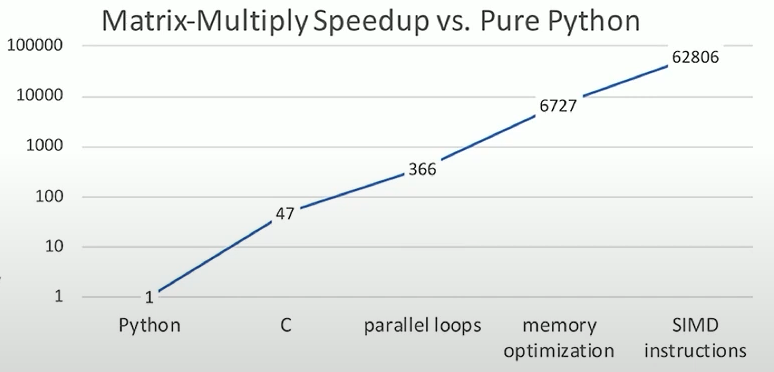
\includegraphics[width=0.75\linewidth]{matrixmul.png}
            \caption{Matrix multiplication in Python vs. C. Source: Emery D. Berger, University of Massachusetts Amherst. \textit{Triangulating Python Performance Issues with SCALENE}. \textbf{OSDI '23}.}
        \end{figure}
    \end{frame}

    \begin{frame}{Why Python?}
        \begin{columns}
            \begin{column}{0.5\linewidth}
                \begin{outline}
                    \1 Each time Python executes a line of code, it must:
                        \2 \textbf{Read} the line of code, parse it, and convert it to bytecode using the Python interpreter.
                        \2 \textbf{Eval} the bytecode, which is executed by the Python Virtual Machine (PVM).
                        \2 \textbf{Print} the result to the console or return it to the calling function.
                \end{outline}
            \end{column}
            \begin{column}{0.5\linewidth}
                \begin{figure}[H]
                    \centering
                    
\includegraphics[width=0.9\linewidth]{python.png}
                \end{figure}
            \end{column}
        \end{columns}
    \end{frame}

    \begin{frame}{Why Python?}
        \begin{outline}
            \1 Curiously, Python was not designed for high-performance computing:
                \2 Pythonic loops are ~40x slower than C loops, and ~60,000x slower than SIMD parallelism.
                \2 Global Interpreter Lock (GIL) prevents true parallelism.
                \2 Python is dynamically typed, which can lead to runtime errors that would be caught at compile time in C.
                \2 Mystery-meat data structures:
                    \3 C \texttt{sizeof(int) == 4} \quad vs. \quad Python \texttt{sys.getsizeof(1) == 28}
                    \3 C \texttt{sizeof(list<int>) == 24} \quad vs. \quad Python \texttt{sys.getsizeof([]) == 56}
                    \3 C \texttt{sizeof(map<int,int>) == 24} \quad -- \quad Python \texttt{sys.getsizeof(\{\}) == 64}
        \end{outline} 
    \end{frame}

    \begin{frame}{Why Python?}
        \begin{figure}[H]
            \centering
            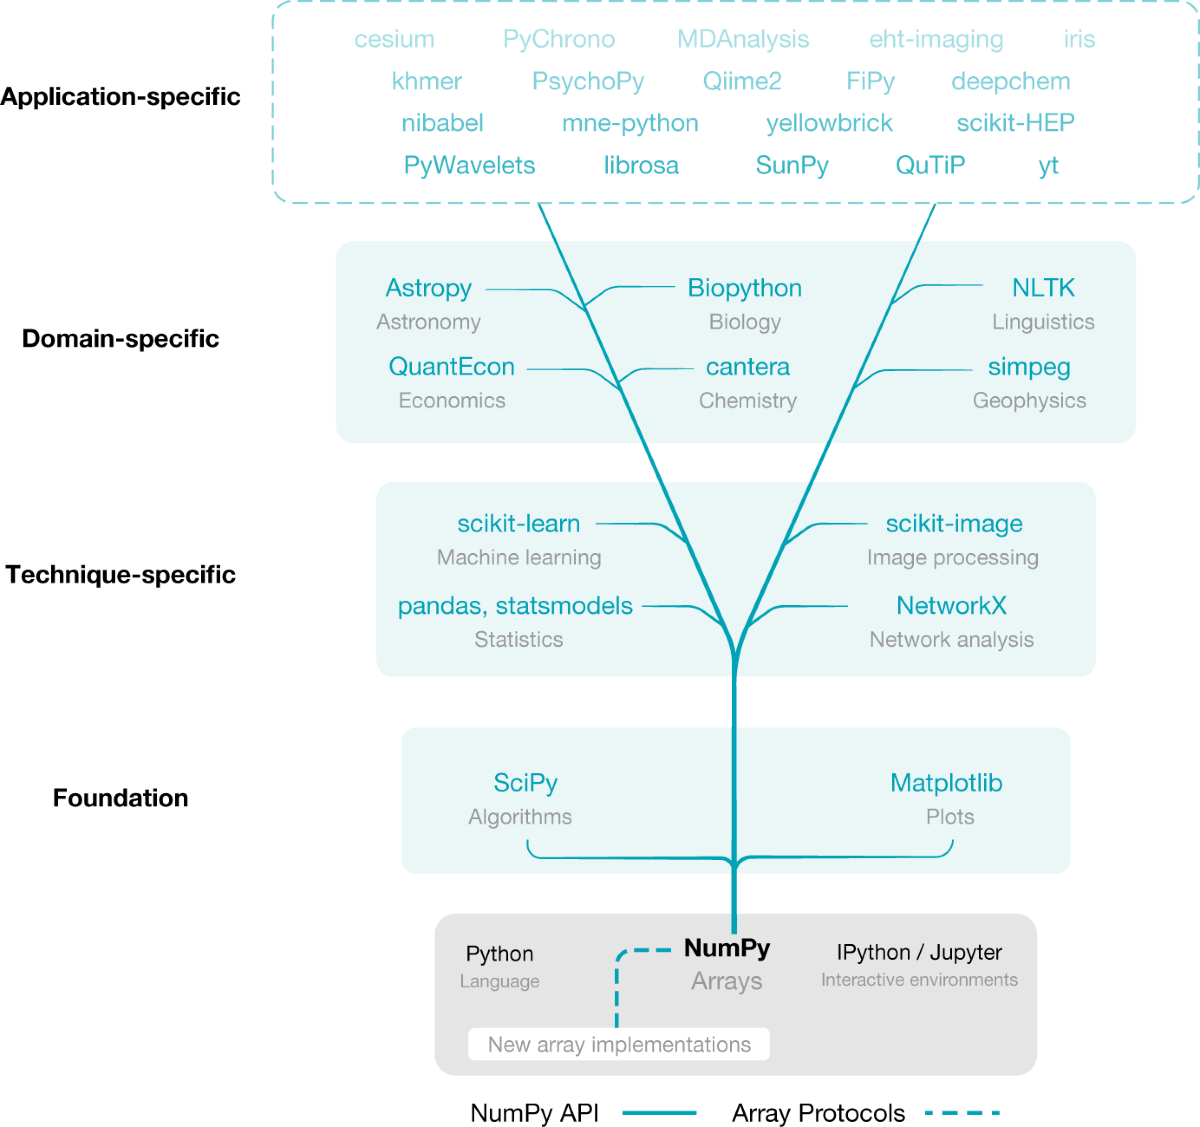
\includegraphics[width=0.40\linewidth]{numpy.png}
            \caption{NumPy provides a high-performance multidimensional array object and is the basis for many projects. Source: Harris, C. et al. \textit{Array programming with NumPy}. \textbf{Nature} 585, 357-362 (2020).}
        \end{figure}
    \end{frame}

    \begin{frame}{Why Python?}
        \begin{outline}
            \1 Despite these drawbacks, Python is the most popular language for scientific computing.
                \2 Python is easy to read and write, and has a large standard library.
                \2 The Python Package Index (PyPI) has over 300,000 packages.
                \2 Data science and machine learning libraries: NumPy, SciPy, TensorFlow, PyTorch, etc. 
                    \3 None of which use Python for performance-critical code.
            \1 Python is a glue language:
                \2 Python is used to call C, C++, Fortran, CUDA, and other languages
                \2 Python is used to orchestrate complex workflows.
                \2 Python is used to prototype and test algorithms.
            \1 A Python developer's real job is to wrap a lower-level languages and generalize them.
        \end{outline}
    \end{frame}

    \begin{frame}{Why Python?}
        \centering
        \Huge Python is not a high performance language,\\
        but it \textit{is} a high productivity language.
    \end{frame}

    \begin{frame}{Python and Package Management}
        \begin{outline}
            \1 Historically, Python package management was an afterthought, and was done manually with zip files or tarballs.
                \2 Guido ultimately wanted a simple and easy-to-use language, and didn't care about package management.
            \1 In 2008, Ian Bicking (who also wrote \texttt{venv}) developed the Python Package Index (PyPI) to host Python packages and introduced \texttt{pyinstall} which later became \texttt{pip}.
            \1 In 2012, Travis Oliphant and others developed the Anaconda distribution, which includes the \texttt{conda} package manager.
            \1 So, there are two package managers for Python: \texttt{pip} and \texttt{conda}, neither of which are:
                \2 perfect
                \2 compatible
                \2 what the creator of Python intended 
        \end{outline}
    \end{frame} 

    \begin{frame}{Using \texttt{pip}}
        \begin{outline}
            \1 \texttt{pip} uses PyPI (https://pypi.org) or a custom index to install packages from source. 
            \1 \texttt{\$ pip --user install package} 
                \2 installs a \texttt{package} for the current user (into \texttt{\$HOME/.local/lib/python3.x/site-packages}).
            \1 \texttt{\$ pip --user install -r requirements.txt}             \1 \texttt{\$ pip install package==version}
            \1 \texttt{\$ pip install package>=version}
        \end{outline}
    \end{frame}

    \begin{frame}{Using \texttt{pip}}
        \begin{outline}
            \1 Virtual environments are used to isolate Python environments from each other.
            \1 \texttt{venv} is the built-in Python virtual environment manager.
                \2 creates a new Python environment in a directory, and installs the Python interpreter and standard library into that directory.
            \1 Managing virtual environments:
                \2 \texttt{\$ python -m venv myenv}
                \2 \texttt{\$ source myenv/bin/activate} - activates the environment.
                \2 \texttt{\$ deactivate} - deactivates the environment.
            \1 Use \texttt{pip} to install packages into the environment, no \texttt{--user} flag needed, as the environment is isolated.
        \end{outline}
    \end{frame}

    \begin{frame}{Using \texttt{pip}}
        \begin{outline}
            \1 Dependencies are not managed: 
            \2 \texttt{pip install package} installs \texttt{package} and its dependencies
            \2 but does not manage them
            \2 or check them against what else is installed.
            \1 \texttt{pip} can quickly become a mess of conflicting dependencies.
        \end{outline}
    \end{frame}

    \begin{frame}{Using \texttt{conda}}
        \begin{outline}
            \1 \texttt{conda} is a package manager which uses a dependency solver to manage packages with specifiable channels.
            \1 Each conda environment is a directory that contains a specific collection of packages, and can be activated and deactivated.
            \2 \texttt{\$ conda create -n condaenv -c default -c conda-forge python=3.9} 
            \2 \texttt{\$ conda activate condaenv} 
            \2 \texttt{\$ conda deactivate}
            \2 \texttt{\$ conda install package}
        \end{outline}
    \end{frame}

    \begin{frame}{Using \texttt{conda}}
        \begin{figure}[H]
            \centering
            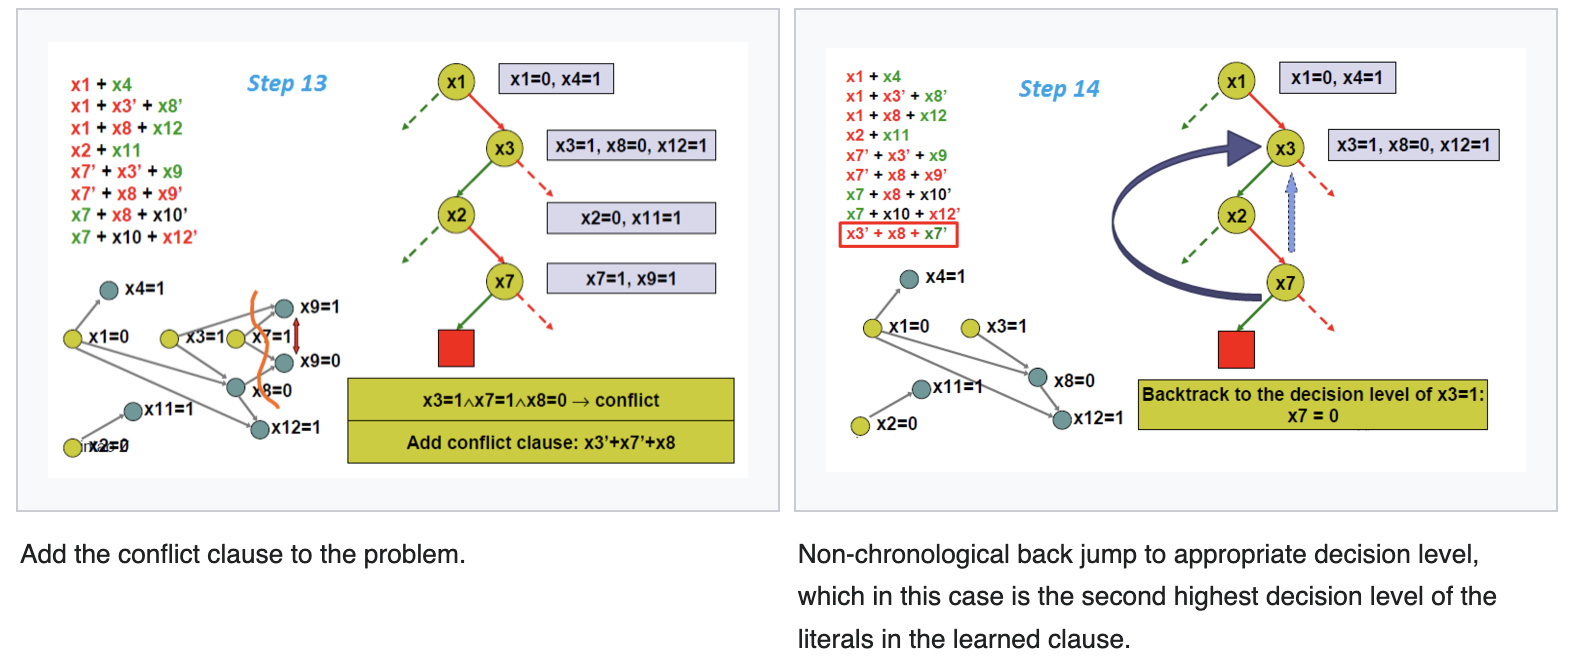
\includegraphics[width=0.75\linewidth]{conda.png}
            \caption{Graph based dependency solver. \ccLogo Tamkin04iut, 2013.}
        \end{figure}
    \end{frame}

    \begin{frame}{Using \texttt{conda}}
        \begin{outline}
            \1 \texttt{\$ conda env export > environment.yml} 
            \1 \texttt{\$ conda env create -n newenv -f environment.yml}   \1 \texttt{\$ conda list} 
            \1 \texttt{conda} can be used alongside \texttt{pip} to manage packages.
                \2 \texttt{\$ conda -n my\_tf -c conda-forge -c nvidia python=3.10} 
                \2 \texttt{\$ conda activate my\_tf}
                \2 \texttt{\$ pip install tensorflow[and-cuda]} 
        \end{outline}
    \end{frame}

    \begin{frame}{Using \texttt{conda}}
        \begin{outline}
            \1 Caveats:
                \2 \texttt{conda} can be slow to resolve dependencies.
                \2 \texttt{conda} can possibly downgrade packages to resolve dependencies (use \texttt{--no-update-deps} if crucial).
                \2 \texttt{conda} comes in several versions: \texttt{conda}, \texttt{mamba}, \texttt{micromamba}, etc. leading to more sharp edges.
        \end{outline}
    \end{frame}

    \begin{frame}{Successful Python on HPC}
        \begin{outline}
            \1 We have a language that is not designed for high-performance computing.
            \1 We have two package managers that are not perfect.
            \1 We have a high-performance computing environment where performance is critical.
        \end{outline}
    \end{frame}

    \begin{frame}{Successful Python on HPC}
        \begin{outline}
            \centering
            \Huge How do we make Python work for HPC?
        \end{outline}
    \end{frame}

    \begin{frame}{Successful Python on HPC}
        \begin{outline}
                \1 Consider the problem and the data. 
                \1 Develop a prototype you can run on small-scale data.
                    \2 Develop a main method which encapsulates the prototype as a function. 
                    \2 Develop a configuration: package management, environment variables, etc.
                \1 Use batch scheduler to run on large-scale data:
                    \2 Use the scheduler to schedule the job with the correct environment variables.
                    \2 Run the main method on the cluster.
                \1 Revise the problem into smaller pieces and run in parallel:
                    \2 Turn loops into functions which can be vectorized, turned into a \textbf{list comprehension}, or \textbf{map-reduced}.
                    \2 Use Dask, joblib, multiprocessing, or mpi4py to run in parallel.
                    \2 Offload mathematics to numpy or CUDA libraries. 
                \1 Analyze the results
        \end{outline}
    \end{frame}

    \begin{frame}{Final Thoughts -- Jupyter Notebooks}
        \begin{outline}
            \1 Jupyter notebooks are a great way to:
                \2 develop and test code.
                \2 document code.
                \2 analyze or visualize data.
                \2 share code that looks great as a portfolio piece.
            \1 Jupyter notebooks are not great for: 
                \2 multi-file projects (use an IDE.)
                \2 parallel computing (unless you really know what you're doing with Dask/multiprocessing.)
                \2 managing dependencies (use a virtual environment.)
                \2 running on a cluster (use a batch scheduler.)
                \2 running in production (use a script.)
        \end{outline}
    \end{frame}

    \begin{frame}{Conclusion}
        \begin{outline}
            \1 Most day-to-day computing is done far away from the metal, but we need to get close to the metal to get the most out of a system.
            \1 To get the maximum performance out of a system, we need to understand the underlying system:
                \2 A typewriter-like interface to the operating system.
            \1 Python wraps lower-level languages and generalizes them, abstracting away the complexity.
                \2 Complexity is moved from the code to understanding the system.
            \1 Development life-cycle: prototype, run on small-scale data, run on large-scale data in parallel, analyze results.
        \end{outline}
    \end{frame}

    \begin{frame}{Live Demo -- Python on CCAST}
        \begin{figure}[H]
            \centering
            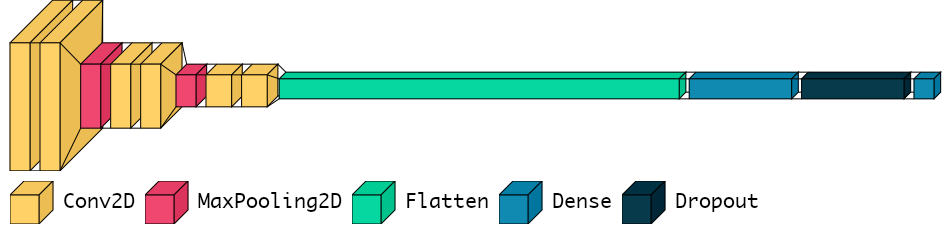
\includegraphics[width=\linewidth]{sequential_model.png}
            \caption{Sequential model of a simple convolutional neural network.}
        \end{figure}
    \end{frame}

    \begin{frame}{Questions?}
        \centering
    \Huge{Questions?}\\ 
    \Huge{Comments?} \\ 
    \Huge{Concerns?}
    \end{frame}

\end{document}
